\newpage
\section{Coordinate Geometry}


Mathematicians in Europe in the 17th Century were just beginning to
come to terms with representing algebraic relations geometrically
using a coordinate plane, and conversely, representing geometric loci
in the (coordinate) plane by algebraic relations.  The solution to
solving this problem for one particular kind of locus was to have
spectacular consequences in astronomy and physics within a century,
and was all tied up with the discovery of calculus by Newton and
Leibniz.

In this activity we will explore the locus of points $(x,y)$ such that
the distance between $(x,y)$ and $(5,0)$ plus the the distance between
$(x,y)$ and $(-4,0)$ is equal to $15$.
\[
%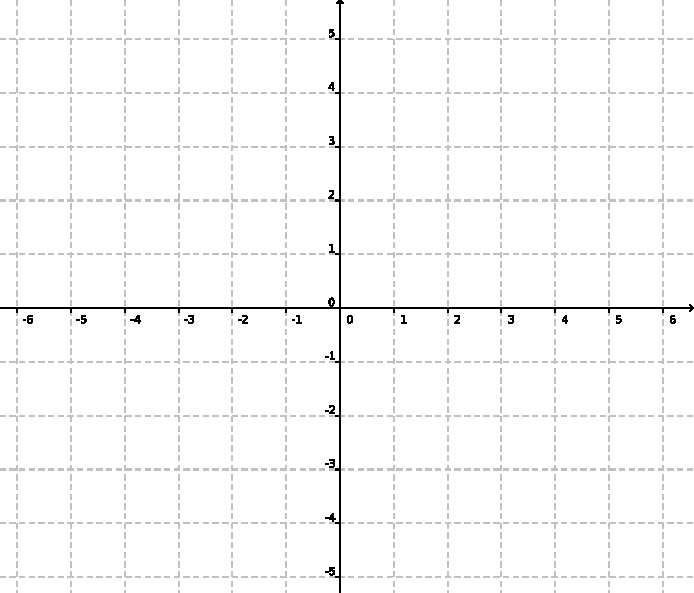
\includegraphics{../graphics/coordPlane.pdf}

\includegraphics{../graphics/complexPlane.pdf}
\]

\begin{prob}
Pick two points, one inside your locus and another outside.
\end{prob}


\begin{prob}
Find four points that are exactly on the locus.  Hint: You can do two
in your head, but you may need the Pythagorean theorem and the
quadratic formula to get the other two.
\end{prob}

\begin{prob} 
Write ``the distance between $(x,y)$ and $(5,0)$ plus the the distance
between $(x,y)$ and $(-4,0)$ is equal to $15$'' as an algebraic
equation.
\end{prob}

Now we will attempt to put the equation above into ``standard form:''
\[
\frac{(x-h)^2}{a^2} + \frac{(y-k)^2}{b^2} = 1
\]

\begin{prob}
To start, isolate one of the square-roots, and square both sides.
\end{prob}

\begin{prob}
Next, isolate the other square-root, and square both sides. 
\end{prob}

\begin{prob}
Complete the square, and get it into standard form! Can you figure out what $a$, $b$, $h$, and $k$ represent?
\end{prob}

